% WISENSE -- replication study of "Tools and Methods for Achieving Wi-Fi Sensing
% in Embedded Devices" (Sensors 2025). Working draft.
%
% Build:  pdflatex wisense_replication && bibtex wisense_replication
%         && pdflatex wisense_replication && pdflatex wisense_replication
% Figures: python -m tools.make_figures   (from WISENSE/)
%
% Every number in this draft comes from a file in WISENSE/ (artifacts/, data logs,
% tools/ outputs); see the Reproducibility section. Lines marked TODO need input.

\documentclass[journal]{IEEEtran}

\usepackage{cite}
\usepackage{amsmath,amssymb}
\usepackage{graphicx}
\usepackage{array}
\usepackage{url}
\usepackage{xcolor}
\usepackage[hidelinks]{hyperref}
\usepackage{tikz}
\usetikzlibrary{positioning,arrows.meta,fit}

\newcommand{\todo}[1]{\textcolor{red}{[TODO: #1]}}

\begin{document}

\title{Reproducing Embedded Wi-Fi Sensing for Human Activity Recognition:\\
A Replication Study on ESP32 Hardware}

\author{Swastik~Kumar,
        Deepak~Kumar,
        Satvik~Rastogi,
        Vansh~Sharma,
        and~Neeru~Jindal%
\thanks{The authors are with the Department of Electronics and Communication
Engineering, Thapar Institute of Engineering \& Technology, Patiala, Punjab 147004,
India. N.~Jindal is an Assistant Professor in the department
(e-mail: skumar6\_be24@thapar.edu; dkumar1\_be24@thapar.edu;
srastogi\_be24@thapar.edu; vsharma4\_be24@thapar.edu; neeru.jindal@thapar.edu).
(Corresponding author: Neeru Jindal.)}}

% Target: IEEE Sensors Journal (IEEEtran journal class).
\markboth{IEEE Sensors Journal, Vol.~XX, No.~XX, Month~2026}%
{Kumar \MakeLowercase{\textit{et al.}}: Reproducing Embedded Wi-Fi Sensing}

\maketitle

\begin{abstract}
Wi-Fi channel state information (CSI) collected on low-cost microcontrollers is an
attractive basis for privacy-preserving human activity recognition (HAR). A recent
study reported a complete embedded pipeline---CSI capture on ESP32 devices, empirical
mode decomposition (EMD) augmentation, and an LSTM-embedded DenseNet running on an
ESP32-S3---with 92.43\% accuracy in 127~kB. We reproduce this work from its public
release, which provides data, collection firmware and trained models but no training,
inference or deployment code. We rebuild the model weight-exactly, recover the
held-out subjects, train with the published hyperparameters for the full 300 epochs,
and rebuild the two-board CSI collection system. Under the original protocol our model
reaches 94.56\% per-subcarrier and 97.10\% majority-vote accuracy in floating point
and 90.87\% when quantized to 8 bits for the single-subcarrier on-device path,
statistically indistinguishable from the released model except for a 2.1-point
gain in floating-point per-subcarrier accuracy. The replication also surfaces several undisclosed
details that materially affect the reported numbers: synthetic training samples are
built from the test subjects' recordings; the model is trained and evaluated per
subcarrier; five specific subcarriers are unusable; the headline 8-bit figure equals
the released model's floating-point score; and the released quantized model occupies
322~kB rather than 127~kB. In a new room, the model falls to near chance (26.8\%
per subcarrier) and is not recovered by fine-tuning or by the original augmentation;
a model-free motion-energy analysis shows that most of the signal variation there is
not caused by the subject. We release the reconstructed pipeline, host-verified
embedded preprocessing and a PlatformIO build of the collection firmware to support a
leak-free re-evaluation.
\end{abstract}

\begin{IEEEkeywords}
Channel state information, ESP32, human activity recognition, reproducibility,
TinyML, Wi-Fi sensing, data leakage.
\end{IEEEkeywords}

% ===================================================================================
\section{Introduction}
% ===================================================================================

\IEEEPARstart{W}{i-Fi} sensing infers human presence and motion from the way a body
perturbs radio propagation between a transmitter and a receiver~\cite{ma2019survey},
and has been used to recognize everyday activities~\cite{wang2015carm}.
The fine-grained quantity used for this is channel state information (CSI): the
per-subcarrier complex channel estimate that an OFDM receiver computes for every
packet. Early CSI work depended on specific network cards with modified
firmware~\cite{halperin2011tool}; the ESP32 family later made CSI available on
microcontrollers costing a few dollars~\cite{hernandez2020esp32}, opening the way to
sensing systems that capture \emph{and} classify on the device, with no camera and no
cloud.

Armenta-Garcia~\textit{et~al.}~\cite{armenta2025tools} presented such a system: a
configurable CSI collection tool for a pair of ESP32 boards, a 22-subject dataset of
five activities, EMD-based data augmentation, and a reduced LSTM-embedded
DenseNet~\cite{huang2017densenet,hochreiter1997lstm} deployed with TensorFlow Lite
Micro~\cite{david2021tflm} on an ESP32-S3. They reported 92.43\% accuracy at 232~ms
per inference in 127~kB of memory, and released the data, collection firmware and
trained models under an open licence~\cite{armenta2025repo}.

This paper is a replication of that work. Our goal was practical: to stand up the
same pipeline on our own hardware as a basis for further research. Doing so required
reconstructing every component that was not released---training, preprocessing for
inference, quantization, and on-device inference---and, in the process, exposed
details of the original evaluation that are absent from the paper but change how its
numbers should be read. Data leakage of this kind is a known source of irreproducible
results in machine-learning-based science~\cite{kapoor2023leakage}.

Our contributions are:
\begin{enumerate}
\item A complete, open reconstruction of the pipeline, with the model architecture
      verified \emph{weight-exactly} against the released checkpoints and the
      held-out subjects recovered exactly from the released training array.
\item A full-budget reproduction under the original protocol (300 epochs, published
      hyperparameters) that matches the released model, with paired significance
      tests.
\item Six findings about the original evaluation and artefacts
      (Section~\ref{sec:findings}), including test-subject leakage through
      augmentation and the identity of the unnamed ``problematic'' subcarriers.
\item A working reproduction of the two-board ESP32 CSI collection system, with the
      configuration and robustness fixes the released firmware needs, and embedded
      preprocessing verified bit-exactly against the host implementation.
\item A cross-environment test in a new room, with fine-tuning, augmentation, gain
      normalization and a fit-check diagnostic, showing that the original pipeline
      does not transfer and why.
\end{enumerate}

% ===================================================================================
\section{Related Work}
\label{sec:related}
% ===================================================================================

\emph{CSI-based activity recognition.} Surveys trace Wi-Fi sensing from early
model-based systems to deep learning~\cite{ma2019survey,miao2025survey}. CARM related
CSI dynamics to body movement speed for activity recognition~\cite{wang2015carm}, and
SenseFi benchmarked deep architectures across public Wi-Fi sensing
datasets~\cite{yang2023sensefi}. Most of this work used network cards with modified
firmware~\cite{halperin2011tool} and offline classification on a PC or GPU.

\emph{Microcontroller platforms.} The ESP32 CSI Tool made per-packet CSI available on
ESP32 microcontrollers~\cite{hernandez2020esp32}, and Espressif's own ESP-CSI
framework provides collection and processing examples~\cite{espressif_esp_csi}. ESP32
hardware has since been used for through-wall activity recognition with an ESP32-S3
and a directional antenna~\cite{strohmayer2023throughwall} and for a public dataset of
ten activities by eight volunteers in line-of-sight and non-line-of-sight
setups~\cite{lim2024esp32dataset}. These works classify on a host, whereas
Armenta-Garcia~\textit{et~al.}~\cite{armenta2025tools} report the complete chain on
ESP32 devices, including on-device inference, and release its data and models; this
combination is why we chose to reproduce it.

\emph{Cross-domain operation.} CSI patterns depend on room, position and person, so a
model trained in one environment often fails in another. Widar3.0 addressed this with
a domain-independent velocity feature and reported 82.6--92.4\% cross-domain gesture
accuracy without retraining~\cite{zheng2019widar3}; recent surveys list data
augmentation and domain adaptation as the main remedies~\cite{miao2025survey}. The
system we reproduce was evaluated in a single room, and Section~\ref{sec:room} tests
it in a second.

\emph{Receiver gain.} Automatic gain control scales the amplitudes of an entire packet
and is a known source of amplitude variation unrelated to the scene. ESP-CSI provides a
mode that fixes the receiver gain~\cite{espressif_esp_csi}; where gain cannot be fixed
or read, dividing each packet's amplitudes by their mean removes the common factor. We
evaluate the latter in Section~\ref{sec:room}.

\emph{Leakage and reproducibility.} Kapoor and Narayanan catalogue data leakage as a
pervasive cause of irreproducible results in machine-learning-based
science~\cite{kapoor2023leakage}. In activity recognition the usual safeguard is a
subject-independent split; Finding F1 shows how augmentation can defeat it even when
the split itself is correct.

% ===================================================================================
\section{The Original System}
\label{sec:original}
% ===================================================================================

\subsection{Data Collection}
Two ESP32 boards act as transmitter (Tx) and receiver (Rx) on a 20~MHz channel. The
Rx operates as an access point; the Tx joins it and sends UDP packets at a configured
rate, and the Rx reports the CSI estimated for each packet from the Tx's MAC address.
With legacy (non-HT) packets the CSI buffer is 128 bytes: 64 subcarriers as
interleaved signed 8-bit imaginary/real pairs. Data leave the Rx over USB serial,
GPIO UART or an SD card, in ASCII or binary form; the authors report an empirical
ceiling of about 85 packets/s for binary output over USB.

\subsection{Dataset}
Twenty-two volunteers performed five activities---fall (FA), get up (GU), lie down
(LD), sit down (SD) and walk (WA)---about 15 times each for 20~s at 50 packets/s in a
computer laboratory, giving 1{,}647 recordings. The released raw files contain
between 866 and 1{,}001 packets each (median 988).

\subsection{Preprocessing and Augmentation}
CSI amplitude is computed per subcarrier, the DC null and guard-band subcarriers are
removed (52 remain), and each recording is truncated to its first 850 packets. The
paper states that 47 subcarriers were finally used and that a single subcarrier with
the highest variance is selected for deployment. For augmentation, ensemble
EMD~\cite{huang1998emd,wu2009eemd} with 100 trials decomposes each subcarrier into
seven intrinsic mode functions plus a residue; a synthetic sample sums the
even-indexed modes of one recording with the odd-indexed modes of another recording
of the same subject and activity. The paper reports 11{,}513 synthetic samples from
1{,}198 real training recordings.

\subsection{Model and Deployment}
The ``LSTM-embedded DenseNet'' replaces DenseNet's 2-D convolutions with 1-D ones,
uses four dense blocks of 3, 6, 12 and 8 layers with growth rate 11, and inserts a
32-unit LSTM before global pooling (122{,}383 parameters). A larger variant with
DenseNet-121 block sizes and a 128-unit LSTM has 437{,}234 parameters. Training uses
Adam at $10^{-4}$, batch size 32 and 300 epochs. The models are quantized to 8 bits
and run under TensorFlow Lite Micro on an ESP32-S3 with external PSRAM.
Table~\ref{tab:reported} lists the reported results.

\begin{table}[!t]
\caption{Results Reported in~\cite{armenta2025tools}}
\label{tab:reported}
\centering
\setlength{\tabcolsep}{4pt}
\begin{tabular}{lcccc}
\hline
Model & Float & 8-bit & Latency & Memory\\
\hline
LSTM-Emb.\ DenseNet & 97.33\% & 92.43\% & 232 ms & 127 kB\\
LSTM-DenseNet121    & 97.55\% & 95.55\% & 817 ms & 277 kB\\
\hline
\multicolumn{5}{l}{\footnotesize 8-bit figures: one subcarrier. All 47 subcarriers:}\\
\multicolumn{5}{l}{\footnotesize 93.32\%, 10{,}904~ms.}
\end{tabular}
\end{table}

% ===================================================================================
\section{Replication Methodology}
\label{sec:method}
% ===================================================================================

\subsection{Released Material}
The authors' repository~\cite{armenta2025repo} contains the raw CSI dataset, the
collection firmware, scripts for amplitude extraction, EMD and dataset construction,
the two trained Keras models with their 8-bit TFLite conversions, and the array of
real training samples. It contains no training script, no inference or
preprocessing code for deployment, no ESP32-S3 firmware and no firmware build
configuration.

\subsection{Recovering the Split}
The dataset-construction script holds out ``the last six'' subjects of an operating
system directory listing, an order that is platform dependent. We matched each of the
1{,}198 samples in the released training array to a raw recording by correlation
of the full $52 \times 850$ amplitude matrix. Every sample matched a distinct
recording with 100\% label agreement, and the six subjects absent from the array---s4
to s9---are the held-out set: 449 recordings, with per-class training and test counts
identical to the paper's.

\subsection{Recovering the Architecture}
The released Keras model files embed their graph configuration. We rebuilt both
models from it with identical layer names and verified the reconstruction by loading
the authors' trained weights layer by layer and requiring numerically identical
outputs. Two details differ from a conventional DenseNet: transition layers output a
fixed five channels---the 0.5 compression factor is applied to the growth rate,
$\lfloor 11 \times 0.5 \rfloor = 5$, not to the channel count---and transitions have no
ReLU. The LSTM is unrolled, as TensorFlow Lite Micro requires. Both variants
reproduce the reported parameter counts exactly.

\subsection{Recovering the Input}
Both released models take a $(850, 1)$ input, but neither the code nor the paper
states how the single subcarrier is chosen. We probed the released small model with
every one of the 52 subcarriers of every held-out recording
(Section~\ref{sec:findings}, Fig.~\ref{fig:subcarriers}); this determined both the
training regime and the set of usable subcarriers.

\subsection{Training}
Following the probe, every usable subcarrier of every recording is a separate
$(850, 1)$ sample. The augmentation reproduces the authors' scripts exactly (EEMD via
PyEMD~\cite{laszuk2017pyemd}, 100 trials, noise seed 5, 7 modes plus residue, all within-subject, within-activity
pairs), including their use of all 22 subjects; we call this the \emph{paper
protocol}. A \emph{clean protocol} that augments only training subjects is
implemented but not yet evaluated at full budget (Section~\ref{sec:discussion}).

EEMD of $1{,}647$ recordings $\times$ 47 subcarriers (77{,}409 series of 850 samples)
took about 5~s per series, over a day of wall-clock time on a 10-core laptop CPU;
EEMD is CPU-bound and does not benefit from a GPU. The resulting pool has 597{,}417 samples: 56{,}306 real and 541{,}111 synthetic.
The synthetic count is exactly $11{,}513 \times 47$, matching the paper's
11{,}513 synthetic recordings.

Training used the published hyperparameters---Adam with learning rate $10^{-4}$,
batch 32, categorical cross-entropy, 300 epochs, each a full shuffled pass of
18{,}669 batches---on one NVIDIA T4 GPU (Kaggle, TensorFlow 2.20). Because sessions are
limited to 12~h, training ran in three sessions resumed from per-epoch checkpoints
that include optimizer state (Fig.~\ref{fig:training}), about 23~GPU-hours in total.
No checkpoint selection was performed: the reported model is the one after epoch
300.

\subsection{Quantization and Scoring}
Models are converted with full-integer post-training quantization~\cite{jacob2018quant}
(uint8 input and output, int8 internally), calibrated on 300 randomly drawn
training-subject samples. We report three scorings of the held-out subjects:
\begin{itemize}
\item \emph{per subcarrier}: each of the 47 subcarriers of each recording classified
      independently (21{,}103 decisions);
\item \emph{one subcarrier}: per recording, only the subcarrier with the largest
      variance of its min--max normalized amplitude among the 47---the on-device
      path, one inference per window;
\item \emph{vote}: majority vote over the 47 per-subcarrier decisions.
\end{itemize}

\subsection{Hardware Reproduction}

\begin{figure*}[!t]
\centering
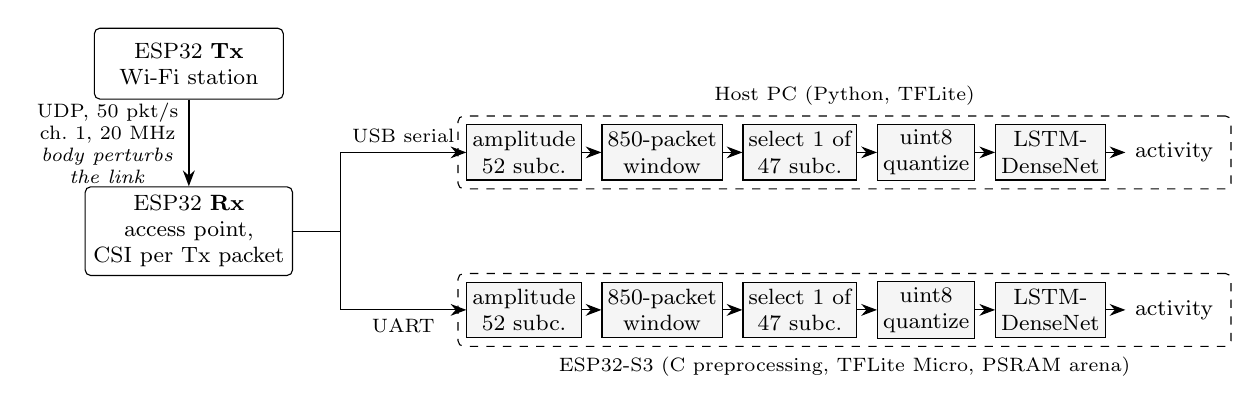
\begin{tikzpicture}[
  font=\footnotesize, >={Stealth[length=2mm]},
  box/.style={draw, rounded corners=2pt, align=center, minimum height=9mm, inner sep=3pt},
  stage/.style={draw, align=center, minimum height=7mm, inner sep=2pt, fill=black!4},
  lbl/.style={align=center, font=\scriptsize}]
\node[box, minimum width=24mm] (tx) {ESP32 \textbf{Tx}\\ Wi-Fi station};
\node[box, minimum width=24mm, below=11mm of tx] (rx) {ESP32 \textbf{Rx}\\ access point,\\ CSI per Tx packet};
\draw[->, thick] (tx) -- node[lbl, left] {UDP, 50 pkt/s\\ ch.~1, 20~MHz\\ \emph{body perturbs}\\ \emph{the link}} (rx);

\node[stage, right=22mm of rx, yshift=10mm] (a1) {amplitude\\ 52 subc.};
\node[stage, right=2.5mm of a1] (a2) {850-packet\\ window};
\node[stage, right=2.5mm of a2] (a3) {select 1 of\\ 47 subc.};
\node[stage, right=2.5mm of a3] (a4) {uint8\\ quantize};
\node[stage, right=2.5mm of a4] (a5) {LSTM-\\DenseNet};
\node[right=2.5mm of a5] (o1) {activity};
\foreach \p/\q in {a1/a2,a2/a3,a3/a4,a4/a5,a5/o1} \draw[->] (\p) -- (\q);
\node[draw, dashed, rounded corners=2pt, inner sep=3pt, fit=(a1)(o1),
      label={[lbl]above:Host PC (Python, TFLite)}] (host) {};

\node[stage, right=22mm of rx, yshift=-10mm] (b1) {amplitude\\ 52 subc.};
\node[stage, right=2.5mm of b1] (b2) {850-packet\\ window};
\node[stage, right=2.5mm of b2] (b3) {select 1 of\\ 47 subc.};
\node[stage, right=2.5mm of b3] (b4) {uint8\\ quantize};
\node[stage, right=2.5mm of b4] (b5) {LSTM-\\DenseNet};
\node[right=2.5mm of b5] (o2) {activity};
\foreach \p/\q in {b1/b2,b2/b3,b3/b4,b4/b5,b5/o2} \draw[->] (\p) -- (\q);
\node[draw, dashed, rounded corners=2pt, inner sep=3pt, fit=(b1)(o2),
      label={[lbl]below:ESP32-S3 (C preprocessing, TFLite Micro, PSRAM arena)}] (s3) {};

\draw[->] (rx.east) -- ++(6mm,0) |- node[lbl, pos=0.75, above] {USB serial} (a1.west);
\draw[->] (rx.east) -- ++(6mm,0) |- node[lbl, pos=0.75, below] {UART} (b1.west);
\end{tikzpicture}
\caption{The reproduced system. The Tx sends packets to the Rx, which reports the CSI of
each one. Classification runs either on a host PC or on an ESP32-S3; both paths apply
the same preprocessing, verified bit-exactly between the Python and C implementations.
The ESP32-S3 path is implemented and host-tested but not yet measured on hardware.}
\label{fig:system}
\end{figure*}

Fig.~\ref{fig:system} shows the reproduced system. We built the collection system with
two ESP32-D0WD-V3 development boards, one with a
CP210x and one with a CH340 USB bridge. The released firmware ships without an
ESP-IDF configuration; we built it with PlatformIO (ESP-IDF~5.5) and supplied the
settings it cannot run without: CSI support enabled in the Wi-Fi driver (it is
compiled out by default), the custom partition table the 1.4~MB application requires,
and a 1~kHz FreeRTOS tick. We also patched the configuration-reset handler, which
erased the stored configuration on any falling edge of GPIO0. On development boards
GPIO0 is driven by the USB-serial auto-reset circuit, and in our tests opening the
serial port was sufficient to erase the configuration; the patch requires the BOOT
button to be held for 3~s. With the Rx streaming binary frames over USB, the host
received 50.1--51.5 valid 128-byte frames per second.

The authors did not release their host capture script or inference firmware. Our
host tool parses the binary stream and writes recordings in the dataset's format.
The ESP32-S3 inference firmware windows incoming frames, selects the subcarrier and
quantizes the input in plain C; this preprocessing is checked against a frozen
output of the Python implementation on a real recording and agrees exactly in the
selected subcarrier, all 850 values and every quantized byte.

% ===================================================================================
\section{Findings About the Original Evaluation}
\label{sec:findings}
% ===================================================================================

\subsubsection*{F1 -- Test subjects leak into training through augmentation}
The authors' synthesis script pairs recordings within every subject directory, and
the dataset-construction script places all synthetic samples in the training set.
Recombined recordings of the six test subjects are therefore trained on. The counts
confirm it: 22 subjects $\times$ 5 activities $\times \binom{15}{2} \approx 11{,}550$
against the reported 11{,}513, whereas the 16 training subjects alone would yield
about 8{,}400. Our reproduction of the scripts yields exactly 11{,}513 synthetic
recordings. Results under this protocol, including ours in Table~\ref{tab:results},
measure accuracy on people whose data contributed to training.

\subsubsection*{F2 -- The model is trained and evaluated per subcarrier}
Although deployment uses a single subcarrier, training treats each subcarrier of
each recording as an independent sample. The reported all-subcarrier latency of
10{,}904~ms is $47 \times 232$~ms: the single-subcarrier model run 47 times.

\subsubsection*{F3 -- The five ``problematic'' subcarriers}
The paper removes five subcarriers without naming them. Fig.~\ref{fig:subcarriers}
shows that on raw subcarriers 1 and 38--41, adjacent to the DC null and the guard
band, the released model scores 20--83\%, against 88--95\% on every other
subcarrier (92--98\% for ours). These subcarriers also have the highest normalized variance, because
they are dominated by noise; a variance-based selection that does not exclude them
selects the worst available input. In our first implementation it selected raw
subcarrier 38 for a held-out recording.

\begin{figure}[!t]
\centering
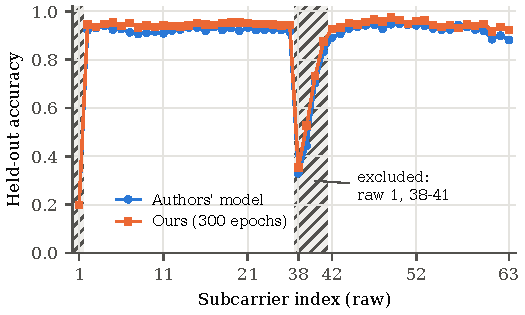
\includegraphics[width=\columnwidth]{figures/fig_subcarriers.pdf}
\caption{Held-out accuracy of each kept subcarrier (paper protocol, float). Hatched
bands mark the five subcarriers excluded to obtain the paper's 47.}
\label{fig:subcarriers}
\end{figure}

\subsubsection*{F4 -- What the headline numbers measure}
Scored as released, the small model reaches 0.9243 per subcarrier in
\emph{floating point}---the value the paper reports as its 8-bit result---while the
released 8-bit model scores 0.9030. The large model's floating-point majority vote,
0.9755, equals the paper's reported floating-point accuracy for that model
(Table~\ref{tab:results}).

\subsubsection*{F5 -- Model size}
The released 8-bit models are 325{,}376 and 779{,}680 bytes; our own conversion of
the small model is 322{,}320 bytes. The reported 127~kB and 277~kB therefore do not
describe the model files; they may refer to the tensor arena, which we have not yet
measured on the device.

\subsubsection*{F6 -- Released firmware is not runnable as shipped}
As described in Section~\ref{sec:method}, the collection firmware requires
configuration that is not provided (CSI support, partition table) and loses its
configuration on USB serial activity.

% ===================================================================================
\section{Results}
\label{sec:results}
% ===================================================================================

Table~\ref{tab:results} compares the released models and ours on the held-out
subjects under the paper protocol, and Table~\ref{tab:stats} tests the differences
between the two small models. Both are scored on the same 449 recordings, so the
comparison is paired: we use McNemar's exact test for the two per-recording scorings
and a recording-level bootstrap (10{,}000 resamples) for 95\% confidence intervals of
all three. Bootstrapping recordings rather than decisions matters for the
per-subcarrier score, because the 47 decisions of one recording are not independent.

Only one difference is significant: floating-point per-subcarrier accuracy, 2.1
points higher for our model (95\% CI +0.2 to +4.0). For the on-device single
subcarrier and for the vote, in floating point and after quantization, every
interval includes zero; our reproduction therefore \emph{matches} the released
model rather than surpassing it. Point estimates for the 8-bit models in
Table~\ref{tab:stats} come from a local TensorFlow~2.18 interpreter and differ by at
most 0.2 points from Table~\ref{tab:results} (TensorFlow~2.20).

\begin{table}[!t]
\caption{Held-out Accuracy, Subjects s4--s9, Paper Protocol}
\label{tab:results}
\centering
\setlength{\tabcolsep}{4pt}
\begin{tabular}{llccc}
\hline
Model & Prec. & Per subc. & One subc. & Vote\\
\hline
Released, small  & float & 0.9243 & 0.9198 & 0.9688\\
                 & uint8 & 0.9030 & 0.8797 & 0.9577\\
Released, large  & float & 0.9544 & 0.9532 & 0.9755\\
                 & uint8 & 0.9474 & 0.9376 & 0.9777\\
Ours, small      & float & 0.9456 & 0.9354 & 0.9710\\
                 & uint8 & 0.8982 & 0.9087 & 0.9510\\
\hline
\multicolumn{5}{l}{\footnotesize Per subcarrier: 21{,}103 decisions; others:}\\
\multicolumn{5}{l}{\footnotesize 449 recordings. Paper protocol: test subjects'}\\
\multicolumn{5}{l}{\footnotesize recordings are in the synthetic training set}\\
\multicolumn{5}{l}{\footnotesize (F1); not a subject-independent score.}
\end{tabular}
\end{table}

\begin{table}[!t]
\caption{Ours Minus Released Small Model, Paired Tests}
\label{tab:stats}
\centering
\setlength{\tabcolsep}{3pt}
\begin{tabular}{llcc}
\hline
Prec. & Scoring & Difference [95\% CI] & McNemar $p$\\
\hline
float & per subcarrier & $+0.021$ [$+0.002$, $+0.040$] & ---\\
      & one subcarrier & $+0.016$ [$-0.016$, $+0.047$] & 0.40\\
      & vote           & $+0.002$ [$-0.020$, $+0.025$] & 1.00\\
uint8 & per subcarrier & $-0.005$ [$-0.027$, $+0.016$] & ---\\
      & one subcarrier & $+0.031$ [$-0.005$, $+0.069$] & 0.12\\
      & vote           & $-0.007$ [$-0.033$, $+0.020$] & 0.74\\
\hline
\multicolumn{4}{l}{\footnotesize CI: recording-level bootstrap. McNemar: exact,
two-sided,}\\
\multicolumn{4}{l}{\footnotesize per recording (not defined per subcarrier).}
\end{tabular}
\end{table}

Per-class recall of our floating-point model per subcarrier is 0.96 (FA), 0.94 (GU),
0.95 (LD), 0.91 (SD) and 0.97 (WA). Quantization costs 4.7 points per subcarrier,
consistent with the paper's reported loss of about 4\%, and falls unevenly: sit-down
recall drops from 0.91 to 0.76, mostly to get-up and fall. The 8-bit model is
322{,}320 bytes.

Enlarging the calibration set does not reduce this loss; it increases it. Re-quantizing
the same trained model with 300, 1{,}000 and 3{,}000 calibration samples gives 0.898,
0.877 and 0.861 per subcarrier, 0.911, 0.891 and 0.878 on the single on-device
subcarrier, and 0.951, 0.940 and 0.940 by vote. The converter sets each activation range
from the extremes it observes, so more samples admit rarer outliers, widen the ranges and
coarsen the 8-bit steps. Recovering the loss therefore needs quantization-aware training
or outlier-robust range estimation rather than more calibration data.

Fig.~\ref{fig:training} shows training accuracy across the three resumed sessions
and held-out scores at the session boundaries. Training accuracy rose smoothly to
0.971 without discontinuities at the resumption points.

\begin{figure}[!t]
\centering
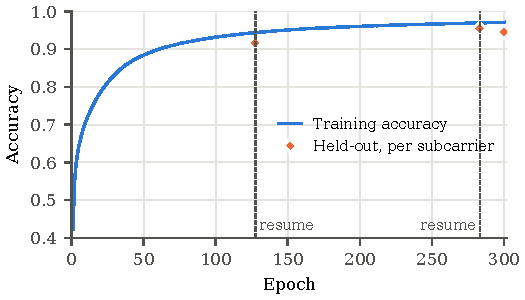
\includegraphics[width=\columnwidth]{figures/fig_training.pdf}
\caption{Training accuracy per epoch over three resumed GPU sessions (dashed lines),
with held-out per-subcarrier accuracy at the end of each session.}
\label{fig:training}
\end{figure}

\subsection{Preliminary Cross-Environment Test}
\label{sec:room}
This test is preliminary: one subject, one session and a link placement that, as shown
below, captured little subject-induced variation. We report it because it quantifies
the failure mode and identifies its cause, not as a measure of achievable
cross-environment accuracy.
On our hardware the host classifies a live 850-packet window every second in about
1.3~ms with the 8-bit model on a laptop CPU. To quantify transfer to a new
environment, one author recorded the five activities and an additional empty-room
class (EM) in a room on our campus, 10 repetitions of 20~s each, with the two boards
of Section~\ref{sec:method} on channel~1, the least congested 2.4~GHz channel at the
site. Four of the 60 recordings were shorter than 850 packets because the stream
stalled, leaving 56. Fine-tuning replaces the output layer with a six-class layer
and trains with the paper's optimizer for 30 epochs; it is scored by stratified
five-fold cross-validation over repetitions, so each recording is tested once by a
model that did not see it. When EEMD augmentation is used, synthetic samples are
built from each fold's training recordings only. Table~\ref{tab:room} gives the
results.

\begin{table}[!t]
\caption{New Room, One Subject, 56 Recordings}
\label{tab:room}
\centering
\setlength{\tabcolsep}{3.5pt}
\begin{tabular}{lcccc}
\hline
Setting & Cls. & Per subc. & One subc. & Vote\\
\hline
Unchanged                 & 5 & 0.268 & 0.239 & 0.304\\
Fine-tuned                & 6 & 0.289 & 0.268 & 0.286\\
Fine-tuned + EEMD         & 6 & 0.241 & 0.196 & 0.268\\
Fine-tuned + gain norm.   & 6 & 0.337 & 0.286 & 0.393\\
From scratch              & 6 & 0.218 & 0.196 & 0.214\\
\hline
Fit, fine-tuned$^\dagger$   & 6 & 0.984 & 0.982 & 1.000\\
Fit, from scratch$^\dagger$ & 6 & 0.221 & 0.232 & 0.179\\
\hline
\multicolumn{5}{l}{\footnotesize Chance 0.20 (5 classes), 0.167 (6). Upper rows:}\\
\multicolumn{5}{l}{\footnotesize five-fold cross-validation.}\\
\multicolumn{5}{l}{\footnotesize $^\dagger$Trained and scored on all 56 recordings.}
\end{tabular}
\end{table}

Unchanged, the paper-trained model is close to chance in the new room and labels
the empty room mostly as get-up or lie-down. Neither fine-tuning nor fine-tuning with
the paper's own augmentation recovers it. The fit check separates the possible
explanations: initialized from the paper-trained weights, the network fits the
recordings it is trained on almost perfectly, so the training procedure works and
the recordings are mutually distinguishable, but what it learns does not transfer to
held-out repetitions. From random initialization it cannot fit them at all, so the
paper-trained representation is what makes the new data learnable.

A model-free measurement explains why. We define motion energy as the mean absolute
packet-to-packet change in amplitude, normalized by its mean, averaged over the 47
subcarriers. In the original dataset walking has the highest median motion energy
(0.211, against 0.180--0.198 for the other activities). In our recordings the empty
room has the highest (0.170, against 0.125--0.151). Dividing each packet's amplitudes
by their mean over subcarriers---which cancels the receiver's automatic gain
changes, since these scale all subcarriers of a packet together---removes about
three quarters of the fluctuation (empty room 0.042, walking 0.039). Fine-tuning on
gain-normalized amplitudes is the best setting we tested (Table~\ref{tab:room}: 0.337
per subcarrier and 0.393 by vote, against a chance level of 0.167), but it remains far
from usable, and in the motion-energy measure the activities still do not stand out
from the empty room. Most of the variation in our recordings is therefore not caused
by the subject, which indicates that link geometry and recording protocol, rather
than the classifier, must be addressed first. Gain normalization is not part of the
original preprocessing and is reported as a candidate addition to it.

% ===================================================================================
\section{Discussion and Limitations}
\label{sec:discussion}
% ===================================================================================

\emph{The reproduced numbers are not subject-independent.} Because of F1, both the
original results and our Table~\ref{tab:results} measure performance on people whose
recombined recordings were trained on. The clean protocol, which removes this
leakage, has so far been run only at a reduced CPU budget (8 augmented subcarriers,
150 epochs of 8{,}000 samples), where it reached 0.49 per-subcarrier accuracy while
still improving; that run is under-trained and not comparable. A full-budget clean
run---the paper's settings, 449{,}978 training samples, two seeds---is in progress
and is the most important pending measurement.

\emph{Variance across runs.} Our paper-protocol result is a single training run.
Repeated runs with different seeds are needed to separate the differences in
Table~\ref{tab:stats} from run-to-run variation.

\emph{Environment dependence.} The original data come from one room, and our test in
a second room (Section~\ref{sec:room}) shows near-chance transfer. That test is itself
limited: one subject, one session, 10 repetitions per class and a single link
geometry. Its motion-energy analysis indicates that our recordings carried little
subject-induced variation, so it does not yet show whether a better-placed link would
transfer. In practical deployments the room is rarely empty; a single Tx--Rx link
mixes the motion of everyone present, and separating concurrent activities of
several people is beyond the single-link design studied here.

\emph{Embedded measurements.} We have not yet measured latency or tensor-arena size
on an ESP32-S3, so the reported 232~ms and 127~kB remain unverified; the firmware is
written and its preprocessing is host-verified, but has not been built and run on
the device.

\emph{Scope of the replication.} We trained the small model only, with one seed and
one calibration set of 300 samples. We used the paper's 47 subcarriers; the released
scripts retain 52, which would add the five noisy subcarriers to training.

% ===================================================================================
\section{Future Work}
% ===================================================================================

\begin{enumerate}
\item Full-budget training and evaluation under the clean protocol.
\item On-device measurement of latency, arena size and accuracy on an ESP32-S3.
\item A second cross-environment collection with controlled link geometry, verified
      beforehand with the motion-energy check; 15 repetitions per class; and a ``no
      event'' class that includes background movement by other people, with each
      activity recorded both alone and with background activity. Recording
      volunteers other than the authors requires ethics approval.
\item Multiple seeds, the large model and a 52-subcarrier variant.
\item Quantization-aware training, since a larger calibration set increases rather than
      reduces the 8-bit loss.
\item Gain normalization evaluated on the original dataset under both protocols, to
      establish whether it helps beyond the new-room setting.
\end{enumerate}

% ===================================================================================
\section{Conclusion}
% ===================================================================================

We reproduced an embedded Wi-Fi sensing pipeline for human activity recognition from
its public release and, under the original protocol, statistically matched the
released model. The replication also showed that the original evaluation trains on
augmented recordings of its test subjects, that the model is trained and scored per
subcarrier, which five subcarriers are excluded and why, and that the headline 8-bit
accuracy and model size do not correspond to the released artefacts. In a second room
the model did not transfer, and neither fine-tuning nor the original augmentation
recovered it; most of the signal variation there was unrelated to the subject. These
details
are necessary to interpret the published numbers and to compare future work fairly.
We release the reconstructed pipeline so that the leak-free evaluation can be
completed and extended.

\section*{Ethics Statement}
The original dataset was collected by Armenta-Garcia~\textit{et~al.} with participants'
informed consent~\cite{armenta2025tools}; we use it as released. The cross-environment
recordings of Section~\ref{sec:room} were made by one of the authors, who was the only
participant and consented to the recording and its publication. Only Wi-Fi channel
measurements were recorded---no video, audio or identifying information. Collection
involving any other participant will be submitted for approval to the institutional
ethics committee of Thapar Institute of Engineering \& Technology before it begins.

\section*{Code and Data Availability}
The code is publicly available under the MIT license at
\url{https://github.com/tetraethylmethane/WISENSE}. It comprises preprocessing,
split recovery, the probe of the released models, augmentation, training,
quantization, evaluation, host capture, the build configuration and patch for the
collection firmware, and the ESP32-S3 firmware with its host tests. The dataset and
original models are those of~\cite{armenta2025repo}.

\section*{Acknowledgment}
We thank Armenta-Garcia~\textit{et~al.} for releasing their data, firmware and
models, without which this replication would not have been possible. GPU time was
provided by Kaggle. This work received no external funding.

\bibliographystyle{IEEEtran}
\bibliography{references}

\end{document}
